\documentclass[a4paper]{article}
\usepackage[spanish]{babel}
\usepackage[utf8]{inputenc}
\usepackage{charter}   % tipografia
\usepackage{graphicx}
%\usepackage{makeidx}
\usepackage{paralist} %itemize inline

%\usepackage{float}
%\usepackage{amsmath, amsthm, amssymb}
%\usepackage{amsfonts}
%\usepackage{sectsty}
%\usepackage{charter}
%\usepackage{wrapfig}
%\usepackage{listings}
%\lstset{language=C}

\usepackage[bookmarks = true, colorlinks=true, linkcolor = black, citecolor = black, menucolor = black, urlcolor = blue]{hyperref} 
\usepackage{color} % para snipets de codigo coloreados
\usepackage{fancybox}  % para el sbox de los snipets de codigo

\definecolor{litegrey}{gray}{0.94}

% \newenvironment{sidebar}{%
% 	\begin{Sbox}\begin{minipage}{.85\textwidth}}%
% 	{\end{minipage}\end{Sbox}%
% 		\begin{center}\setlength{\fboxsep}{6pt}%
% 		\shadowbox{\TheSbox}\end{center}}
% \newenvironment{warning}{%
% 	\begin{Sbox}\begin{minipage}{.85\textwidth}\sffamily\lite\small\RaggedRight}%
% 	{\end{minipage}\end{Sbox}%
% 		\begin{center}\setlength{\fboxsep}{6pt}%
% 		\colorbox{litegrey}{\TheSbox}\end{center}}

\newenvironment{codesnippet}{%
	\begin{Sbox}\begin{minipage}{\textwidth}\sffamily\small}%
	{\end{minipage}\end{Sbox}%
		\begin{center}%
		\vspace{-0.4cm}\colorbox{litegrey}{\TheSbox}\end{center}\vspace{0.3cm}}



\usepackage{fancyhdr}
\pagestyle{fancy}

%\renewcommand{\chaptermark}[1]{\markboth{#1}{}}
\renewcommand{\sectionmark}[1]{\markright{\thesection\ - #1}}

\fancyhf{}

\fancyhead[LO]{Sección \rightmark} % \thesection\ 
\fancyfoot[LO]{\small{Aldasoro Agustina, More \'Angel, Zimenspitz Ezequiel}}
\fancyfoot[RO]{\thepage}
\renewcommand{\headrulewidth}{0.5pt}
\renewcommand{\footrulewidth}{0.5pt}
\setlength{\hoffset}{-0.8in}
\setlength{\textwidth}{16cm}
%\setlength{\hoffset}{-1.1cm}
%\setlength{\textwidth}{16cm}
\setlength{\headsep}{0.5cm}
\setlength{\textheight}{25cm}
\setlength{\voffset}{-0.7in}
\setlength{\headwidth}{\textwidth}
\setlength{\headheight}{13.1pt}

\renewcommand{\baselinestretch}{1.1}  % line spacing


% \setcounter{secnumdepth}{2}
\usepackage{underscore}
\usepackage{caratula}
%\usepackage{url}



% ******************************************************** %
%              TEMPLATE DE INFORME ORGA2 v0.1              %
% ******************************************************** %
% ******************************************************** %
%                                                          %
% ALGUNOS PAQUETES REQUERIDOS (EN UBUNTU):                 %
% ========================================
%                                                          %
% texlive-latex-base                                       %
% texlive-latex-recommended                                %
% texlive-fonts-recommended                                %
% texlive-latex-extra?                                     %
% texlive-lang-spanish (en ubuntu 13.10)                   %
% ******************************************************** %



\begin{document}


\thispagestyle{empty}
\materia{Sistemas Operativos}
\submateria{Primer Cuatrimestre 2015}
\titulo{Trabajo Práctico I}
\subtitulo{Scheduling}
\integrante{Aldasoro Agustina}{86/13}{agusaldasoro@gmail.com}
\integrante{More \'Angel}{931/12}{angel_21_fer@hotmail.com}
\integrante{Zimenspitz Ezequiel}{155/13}{ezeqzim@gmail.com}

\maketitle
\newpage

\thispagestyle{empty}
\vfill
\begin{abstract}
En el presente trabajo se describe la problemática de ...
\end{abstract}
\newpage

\thispagestyle{empty}
\vspace{3cm}
\tableofcontents
\newpage


%\normalsize
\newpage
\section{Parte I}

\subsection{Ejercicio 1: TaskConsola}
\textit{Programar un tipo de tarea TaskConsola, que simular\'a una tarea interactiva. La tarea debe realizar n llamadas bloqueantes, cada una de una duraci\'on al azar entre bmin y bmax (inclusive). La tarea debe recibir tres par\'ametros: n, bmin y bmax (en ese orden) que ser\'an interpretados como los tres elementos del vector de enteros que recibe la funci\'on.}\\

Al momento de ejecutar la tarea \emph{TaskConsola}, lo que realiza nuestro algoritmo es \emph{uso_IO} \textcolor{red}{(sistema operativo???)} n veces, eligiendo cada vez un n\'umero al azar -mediante la funci\'on rand()- entre bmin y bmax.



\subsection{Ejercicio 2: Ejecuci\'on de tres tareas}
\textit{Escribir un lote de 3 tareas distintas: una intensiva en CPU y las otras dos de tipo interactivo (TaskConsola). Ejecutar y graficar la simulaci\'on usando el algoritmo FCFS para 1, 2 y 3 n\'ucleos.}\\

Para observar el comportamiento de un lote de tareas en un scheduler basado en la técnica FCFS
(\textit{First Came, First Served}). Donde cada una se ejecuta en el orden en el que se encuentran $ready$. Se ejecutaron tres tareas distintas. Dos se corresponden el tipo de tarea $TaskConsola$ y la otra solo haciendo uso intensivo del CPU (sin bloqueo). Las tareas utilizadas las siguientes:
	\begin{codesnippet}
	\begin{verbatim}
TaskConsola 4 2 7
TaskCPU 3
@3:
TaskConsola 5 1 10
	\end{verbatim}
	\end{codesnippet}
	
Además para observar como varía el tiempo total (si es que lo hace), se simuló la ejecución para 1, 2 y 3 cores. Dado que en este tipo de Scheduler no hay cambio de contexto ni migración de procesos entre los distintos núcleos los demas parametros no son de importancia.

Los diagramas de Gantt obtenidos fueron los siguientes:\\

 \begin{figure}[h!]
   \begin{center}
 	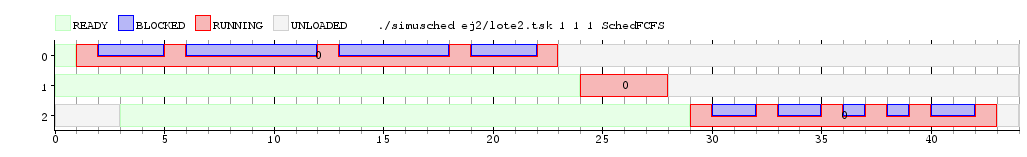
\includegraphics[scale=0.5]{imagenes/ej2/1core.png}
 	\caption{Diagrama de Gantt para la ejecuci\'on del lote de tareas bajo 1 n\'ucleo.}
   \end{center}
 \end{figure} 
 

 \begin{figure}[h!]
   \begin{center}
 	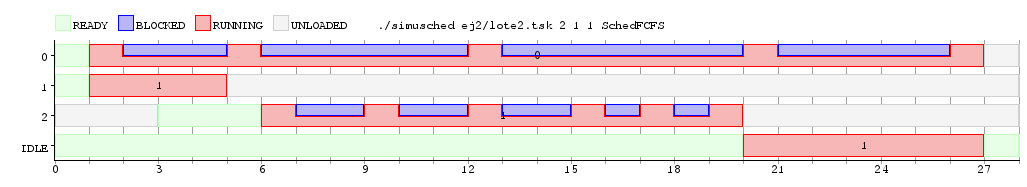
\includegraphics[scale=0.5]{imagenes/ej2/2core.png}
 	\caption{Diagrama de Gantt para la ejecuci\'on del lote de tareas bajo 2 n\'ucleos.}
   \end{center}
 \end{figure} 
 
  \newpage

  \begin{figure}[h!]
   \begin{center}
 	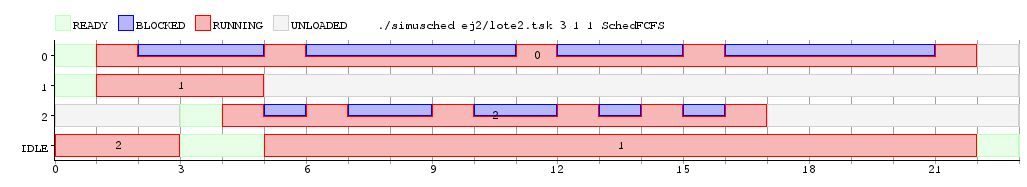
\includegraphics[scale=0.5]{imagenes/ej2/3core.png}
 	\caption{Diagrama de Gantt para la ejecuci\'on del lote de tareas bajo 3 n\'ucleos.}
   \end{center}
 \end{figure} 

\textcolor{red}{Aca habria que hablar un poco y revisar esto: :D}

A partir de los resultados obtenidos en los gráficos anteriores. Podemos observar que el tiempo total varía de acuerdo al número de cores con los que se este simulando. A medida que se incrementa el número el tiempo total disminuye. No solo influyó este factor sino que también, el hecho de que estamos trabajando con un modelo sin desalojo.  
Al trabajar con un solo core debemos esperar que una tarea finalice para que la próxima pueda ser ejecutada. Es decir, se van a ir ejecutando secuencialmente según fueron estando $ready$. \newline
Al aumentar en una unidad el número de core. La primer tarea disponible comenzó a ejecutarse. Dado que aun disponemos de otro core, cuando una segunda tarea paso a estar disponible pudo ser ejecutada al instante por el núcleo adicional. Y cuando uno de estos se desocupó se ejecutó la última tarea. Dado que dos tareas pudieron ejecutarse simultaneamente el tiempo total disminuyó. Aún más cuando se trabajó con 3 cores cada tarea pudo ser ejecutada en un núcleo distinto y dado que ambas podian ser ejecutadas mientras se ejecutaban las otras el tiempo total fue igual al máximo entre $release$ $time_j$ + $c_j$, donde j indica alguna de las tres tares utilizadas y $c_j$ su tiempo de ejecución.   
\newpage

\section{Parte II}


\subsection{Ejercicio 3: Scheduler Round-Robin}

\textit{Completar la implementaci\'on del scheduler Round-Robin implementando los m\'etodos de la clase SchedRR en los archivos sched_rr.cpp y sched_rr.h. La implementaci\'on recibe, como primer par\'ametro, la cantidad de n\'ucleos y a continuaci\'on los valores de sus respectivos quantums. Debe utilizar una \'unica cola global, permitiendo as\'i la migraci\'on de procesos entre n\'ucleos.}\\


Las estructuras de datos con las que vamos a trabajar, en la clase \emph{SchedRR}, son las siguientes:
	\begin{codesnippet}
	\begin{verbatim}
		int cores;
		vector<int> quantums;
		vector<int> quantums_timer;
		vector<int> actuales;
		int siguiente;
		queue< int, deque<int> > cola;
	\end{verbatim}
	\end{codesnippet}
	
	\begin{itemize}
	\item[•]\textbf{cores} es la cantidad de n\'ucleos.
	\item[•]\textbf{quantums} es un vector de \textit{cores} posiciones, que guarda en quantums[i] el valor del quantum asignado al n\'ucleo i.
	\item[•]\textbf{quantus_timer} es un vector, tal que quantus_timer[i] representa el valor del quantum restante para la tarea corriendo en el n\'ucleo i.
	\item[•]\textbf{actuales} vector que indica el PID de la tarea ejecutandose en el núcleo i (actuales[i]). Para los núcleos sin tarea devuelve la constante $IDLE\_TASK$.
	\item[•]\textbf{siguiente} indica el core al que se le debe asignar la siguiente tarea.
	\item[•]\textbf{cola} es la cola de tareas que restan ser ejecutadas.
	\end{itemize}	
	
%\bigskip	
\noindent  Modificamos a la funcion \emph{next} para que reciba un parametro m\'as (enum Motivo \{ TICK, BLOCK, EXIT \}).
	\begin{codesnippet}
	\begin{verbatim}
    int next(int cpu, const enum Motivo m);
	\end{verbatim}
	\end{codesnippet}
		
\subsubsection*{Constructor Scheduler Round-Robin}		

Al construir un Scheduler Round-Robin, se instancian las estructuras de datos de modo que: se le asigna la cantidad de cores correspondientes (con sus respectivos quantums), todas las tareas actuales se definen como Iddle, la cola est\'a vac\'ia y el siguiente n\'ucleo que le corresponde ejecutar es el primero ingresado como par\'ametro.

\subsubsection*{Funci\'on Load}

Recibe el \emph{pid} de una nueva tarea como par\'ametro. Luego, las primeras n tareas (siendo n el número de cores) se distribuyen entre cada core (dado que al inicio tengo n cores disponibles). Una vez alcanda las n distribuciones se encolan los nuevos \emph{pid} en \emph{cola}. Estos seran asignados a los distintos cores con la función $next$ explicada luego.

\subsubsection*{Funci\'on Tick}	

Recibe \emph{cpu} como par\'ametro y el \emph{Motivo}. Dado que se produjo un tick voy a actualizar el quantum (restarle 1) de la tarea en \emph{cpu}, si no es la Iddle (porque esta corre indefinidamente hasta que la desplace otra tarea). 
Si se acab\'o el quantum de la tarea actual (ya sea porque termin\'o o no) o se bloque\'o, voy a querer actualizar la tarea actual. Para esto, invocó a la funci\'on \emph{next()}. La misma devuelve el \emph{pid} de la próxima tarea a ejecutar en \emph{cpu}.

\subsubsection*{Funci\'on Next}	
	
La funci\'on Next tambi\'en va a ser invocada para un s\'olo n\'ucleo \emph{cpu} pasado por par\'ametro.\\
De este modo, si la tarea que se estaba ejecutando previo a la invocaci\'on de \emph{next()} termin\'o de ejecutarse y la cola se encuentra vac\'ia, la tarea que pondr\'a a ejecutar va a ser la Tarea Iddle.
Si la tarea que se estaba ejecutando no termin\'o su ejecuci\'on o se bloqueo, se deber\'a encolar en la cola global de pendientes.
Si todav\'ia no asign\'e una tarea actual para el n\'ucleo cpu, le asigno la primera de la cola d\'andole todo el quantum disponible para el n\'ucleo \emph{cpu}. (Si la cola se encontraba vac\'ia al llamar la funci\'on next() y la tarea ejecut\'andose no hab\'ia conclu\'ido se la encolar\'a para luego volver a asign\'arsela al n\'ucleo).\\
 
\bigskip 
 
 
 \subsection{Ejercicio 4: Ejecuci\'on de lotes de tareas}
 
\textit{Dise\~nar uno o m\'as lotes de tareas para ejecutar con el algoritmo del ejercicio anterior. Graficar las simulaciones y comentarlas, justificando brevemente por qu\'e el comportamiento observado es efectivamente el esperable de un algoritmo Round-Robin.}\\


Para poder observar el comportamiento del Scheduler basado en la metodologia Round Robin evaluamos tres casos.

\subsection{1er caso:}

Ejecutamos el mismo lote de tareas utilizado anteriormente (pág 4), manteniendo los mismos parametros, para asi poder evaluar y comparar un Scheduler basado en Round Robin y otro en FCFS. 

	\begin{codesnippet}
	\begin{verbatim}
TaskConsola 4 2 7
TaskCPU 3
@3:
TaskConsola 5 1 10
	\end{verbatim}
	\end{codesnippet}

Los diagramas de Gantt obtenidos fueron los siguientes:\\


 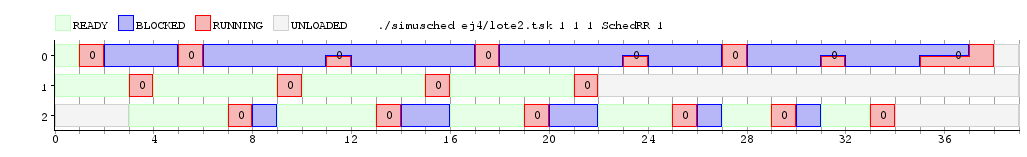
\includegraphics[width=\textwidth,height=3.0in,keepaspectratio
]{imagenes/ej4/1core.png} \newline
\begin {flushleft}
\textbf{Figura 4:} Diagrama de Gantt para la ejecuci\'on del lote de tareas bajo 1 n\'ucleo con Scheduler Round Robin.
\end{flushleft}

  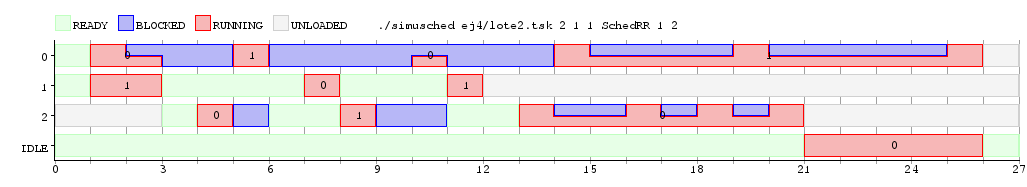
\includegraphics[width=\textwidth,height=3.0in,keepaspectratio
]{imagenes/ej4/2core.png} \newline
\begin {flushleft}
\textbf{Figura 5:} Diagrama de Gantt para la ejecuci\'on del lote de tareas bajo 2 n\'ucleos con Scheduler Round Robin.
\end{flushleft}


  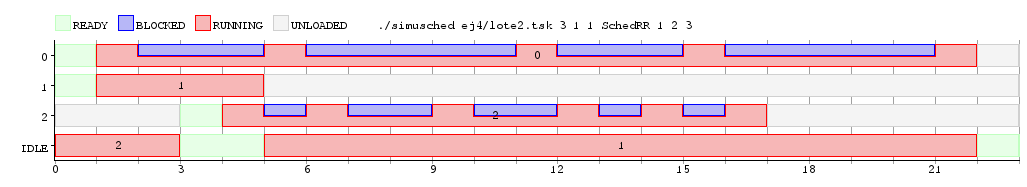
\includegraphics[width=\textwidth,height=3.0in,keepaspectratio
]{imagenes/ej4/3core.png} \newline
\begin {flushleft}
\textbf{Figura 6:} Diagrama de Gantt para la ejecuci\'on del lote de tareas bajo 3 n\'ucleos con Scheduler Round Robin.
\end{flushleft}
 
Apartir de los resultados obtenidos podemos ver que para los gráficos 5 y 6 el tiempo total de ejecución fue el mismo que para las figuras 2 y 3 respectivamente. En estos casos observamos que el tiempo dependió de la tarea TaskConsola 4 2 7. La cual tenia el mayor tiempo de ejecución. Entonces, sin importar el modelo, aunque las otras dos tareas terminaron el procesador tuvo que esperar a que finalice dicha tarea. Un caso interesante para análizar es de la figura 1 y 4. En ambas, solo se utilizaba un núcleo. Pero, en el modelo Round Robin el tiempo de ejecución fue menor. Esto se debe al comportamiento de dicho scheduler que permite cambios de contexto y migración deprocesos. Para el modelo FCFS, había que esperar que una tarea finalice para ejecutar la próxima. Si ésta tenía mucho tiempo de bloqueo entonces ese tiempo se desperciaba. En el modelo Round Robin se pudieron aprovechear esos tiempos para ejecutar las otras tareas. Y dado que la tarea con mayor tiempo de ejecución era del tipo TaskConsola con muchos períodos de bloqueo. El tiempo fue lo suficiente como para ejecutar en su totalidad las otras tareas.  
 \bigskip
 
 \subsection{2do caso:}
 
 Para este caso se creo un nuevo lote de tareas y lo que se busco fue analizar como varía el tiempo total de ejecución, para las mismas, a medida que se cambia el quantum para un total de dos cores.\newline 
 Las tareas que se usaron son las siguientes:\newline
 \begin{codesnippet}
	\begin{verbatim}
TaskConsola 10 2 6
TaskCPU 10
@3:
TaskCPU 7
@2:
TaskConsola 7 4 10
	\end{verbatim}
	\end{codesnippet}

Los resultados obtenidos son:

 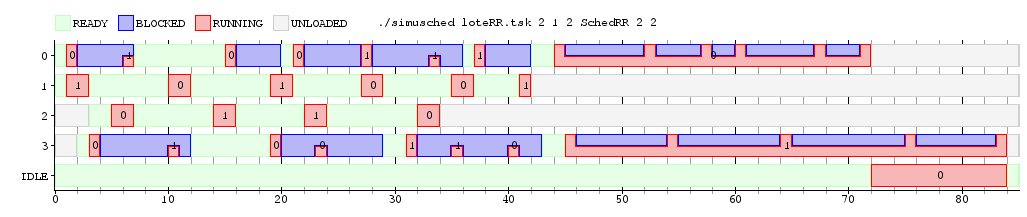
\includegraphics[width=\textwidth,height=3.0in,keepaspectratio
]{imagenes/ej4/eje1.png} \newline
\begin {flushleft}
\textbf{Figura 7:} Diagrama para la ejecuci\'on del lote de tareas bajo 2 n\'ucleos con quantum de 2 y 2 ciclos respectivamente.
\end{flushleft}

 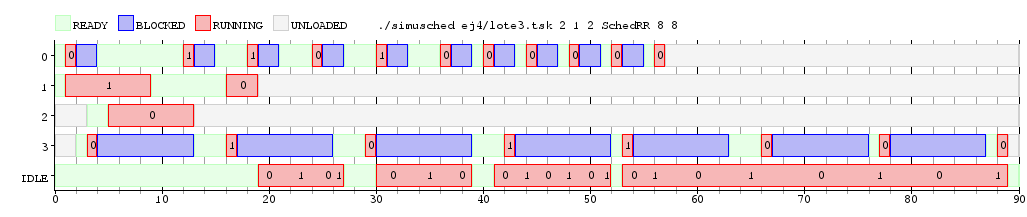
\includegraphics[width=\textwidth,height=3.0in,keepaspectratio
]{imagenes/ej4/eje2.png} \newline
\begin {flushleft}
\textbf{Figura 8:} Diagrama para la ejecuci\'on del lote de tareas bajo 2 n\'ucleos con quantum de 8 y 8 ciclos respectivamente.
\end{flushleft}


 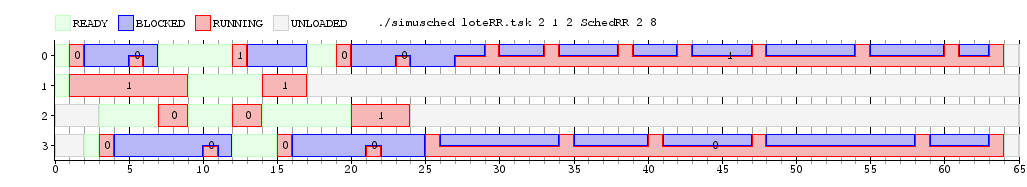
\includegraphics[width=\textwidth,height=3.0in,keepaspectratio
]{imagenes/ej4/eje3.png} \newline
\begin {flushleft}
\textbf{Figura 9:} Diagrama para la ejecuci\'on del lote de tareas bajo 2 n\'ucleos con quantum de 2 y 8 ciclos respectivamente.
\end{flushleft}

Los resultados obtenidos se acercan a lo esperado. Los cuales fueron que para quantums muy chicos, el tiempo de ejecución total aumente frente a otros casos. Lo cual se observa en la figura 7. Principalmente cuando se utilizan quantums muy chicos ocurren muchos cambios de contextos. Si este no es depreciable, AumentandA el tiempo total que el procesador necesita para ejecutar todas las tareas. Luego, al aumentar el quantum de cada core a 8 (figura 8), observamos que el tiempo total fue menor que para el caso anterior. Ya que, se produjeron menos cambios de contexto. Sin embargo, cuando se usó un quantum bajo y otro de mayor ciclo, el tiempo total bajó con respecto al anterior caso. Podemos atribuir este comportamiento al tipo de tareas con el que se trabajamos como se observa, algunas tareas pudieron migrar en este último caso y finalizar su ejecución más rapidamente. Intuyendo, con estos resultados, que quantums de ciclos muy bajos no son beneficiosos. Lo mejor es encontrar un promedio de la cantidad de ciclos para un quantum dado que para valores mas grandes también se observó que puede tardar más con respecto a otros casos.   
 
 \subsection{3er caso:}
 
 En el último caso se observó el comportamiento para un lote  de tarea. A medida que modificabamos el número de núcleos en los que se ejecutaban las mismas.\newline
 Las tareas usadas fueron:
 \begin{codesnippet}
	\begin{verbatim}
TaskCPU 7
@2:
TaskCPU 6
@1:
TaskCPU 10
@3:
TaskCPU 4
	\end{verbatim}
	\end{codesnippet}
	
	Obteniendo los siguientes resultados:

  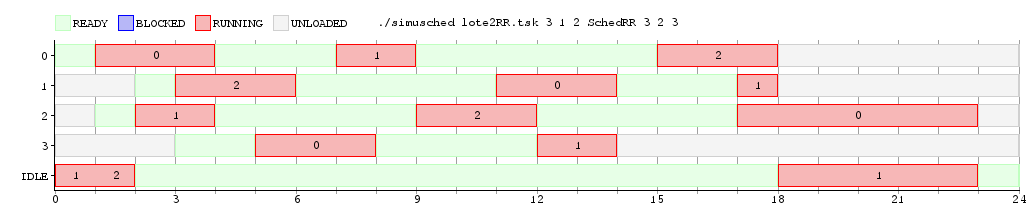
\includegraphics[width=\textwidth,height=3.0in,keepaspectratio
]{imagenes/ej4/eje4.png} \newline
\begin {flushleft}
\textbf{Figura 10:} Diagrama de Gantt para la ejecuci\'on del lote de tareas bajo 3 n\'ucleos con Scheduler Round Robin.
\end{flushleft}




 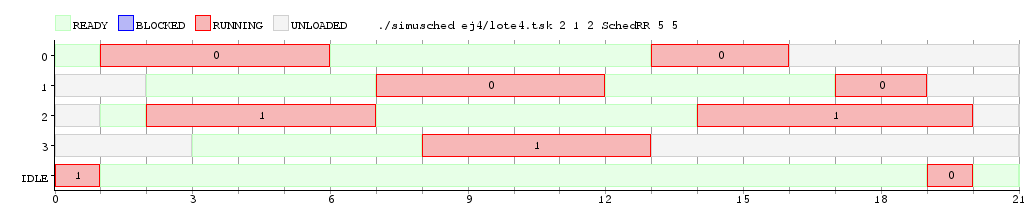
\includegraphics[width=\textwidth,height=3.0in,keepaspectratio
]{imagenes/ej4/eje6.png} \newline
\begin {flushleft}
\textbf{Figura 11:} Diagrama de Gantt para la ejecuci\'on del lote de tareas bajo 2 n\'ucleos con Scheduler Round Robin.
\end{flushleft}
 

En este último caso quisimos comparar el comportamiento de un mismo lote de tareas cuando modificabamos el número de cores en un Scheduler Round Robin. Lo que observamos fue que cuando se contaba con un número mayor de cores las migraciones de procesos fueron mas frecuentes. Dado que estas no son despreciables y de hecho tienen un costo de 2 ciclos. Al producirse en gran cantidad el tiempo total para la finalización de tareas aumentó considerablemente. Como se observa en la figura 10, hay un gran lapso de tiempo entre la ejecución de una misma tarea. Dado que en cada quantum se ejecutaron en un core distinto. En cambio, en la figura 11 no se prudujeron migraciones, y pese a que se contaba con un core menos el tiempo fue menor. Pudiendo concluir que aunque las migraciones de procesos pueden ser provechosas como se observó en el caso 2 (pág 9). Si se producen en exceso pueden perjudicar la perfomance del procesador.  

\newpage

 \subsection{Ejercicio 5: Scheduling algorithms for multiprogramming in a hard-real-time environment}
 
\textit{A partir del art\'iculo Liu, Chung Laung, and James W. Layland. Scheduling algorithms for multiprogramming in a hard-real-time environment. Journal of the ACM (JACM) 20.1 (1973): 46-61.}\newline

Responda:
\begin{enumerate}
\item \textit{¿Qu\'e problema est\'an intentando resolver los autores?}

\item \textit{¿Por qu\'e introducen el algoritmo de la secci\'on 7? ¿Qu\'e problema buscan resolver con esto?}

\item  \textit{Explicar coloquialmente el significado del teorema 7.}

\end{enumerate}

\subsection{a:}

Frente al avance que se venia produciendo en esos años del uso de las computadoras en distintos procesos industriales. Los autores establecieron que esto se iría masificiando aún más. Y que una correcta aplicación solo es posible cuando se tiene un scheduler eficiente y factible. Sobre todo para aquellos usos en los cuales se requerían que las tareas llevadas al cabo se ejecuten dentro de un lapso de tiempo determinado (a lo cual lo llaman \textit{"hard-real-time"}). Ya que en caso contrario, una respuesta tardía podría provocar un efecto no deseado en una aplicación o no sería de interés. Además intentaron desarollar este tema. Ya que como describen, la mayoría de paper, hasta entonces, estaban orientados a contextos en lo que no había una cota de tiempo para llevar a cabo todas las tareas. Y los que habían, hacían uso de varios supuestos, llevando en algunos casos a situaciones irreales. Por lo que plantearon dos modelos de scheduler para tareas en un entorno de \textit{hard-real-time}. Ambos se basan en fijar prioridades para cada una de las tareas pero, uno de manera estática y el otro dinámicamente. Además para mejorar el rendimiento del mismo buscan establecer cotas (cuando es posible) para determinar si es aplicable alguno de los modelos. De manera que no se produzca \textit{overflow} (alguna de las tareas finalice su ejecución después del tiempo límite).


\subsection{b:}
En la sección 7 se introduce un nuevo algoritmo, el cual es para un scheduler basado en asignaciones de prioridades dinámicamente (llamado \textit{The deadline Driven Scheduling}). Lo introducen como una variante al algoritmo presentado anteriormente (para un scheduler con prioridades fijas). Intentando evitar o disminuir algunos de los problemas presentados para dicho modelo. \newline
Una de los problemas a resolver es mejorar las asignaciones de las prioridades. De manera de aprovechar el procesador a un 100\%. De esta forma, este nuevo algoritmo establece que el nuevo modelo nunca va a ejecutar la idle sino, que siempre se va a estar ejecutando alguna tarea. A diferencia del modelo de prioridades fijas, donde la utilización del procesador podía variar de un 70 a un 100\%. Para conseguir esto, se va a aumentar o disminuir la prioridad de una tarea conforme se acerca a su deadline, es decir las prioridades de una misma tarea van a ser modificadas a lo largo de su ejecución. Además, buscaron determinar si un conjunto de tareas evitara producir overflow, con este algoritmo. En el caso del scheduler con prioridades fijas, se estableció una condición para tal motivo (\textit{teorema 4 $^1$}). Pero, la misma solo es necesaria. Para el scheduler presentado en esta sección se desarrollo una nueva condición, \textit{teorema 7}, la cual garantiza que si se cumple entonces es aplicable el algoritmo y en caso contrario, no lo es (el mismo sera explicado en el siguiente punto). 
  
\subsection{c:}

Teorema 7:
\textit {For a given set of m tasks, the deadline driven scheduling algorithm
is feasible if and only if }\newline
 
 \textit {$(C_1/T_1)$ + $(C_2/T_2)$ + . . . + $(C_m/T_m)$ $\leq$ 1 } $^2$\newline

\textit{Siendo $C_i$ el tiempo de ejecuci\'on para una tarea i, 1 $\leq$ i $\leq$ m, y $T_i$ su respectivo per\'iodo.}

En las secciones anteriores, al presente teorema, se determina que la fracción de CPU que utiliza una tarea en el sistema esta dado por $C_i/T_i$ (\textit{the utilization factor}). Lo que se plantea en este teorema es que un scheduler, para una cantidad m de tareas, es factible y por lo tanto realizable sin que se produzca overflow. Cuando la suma del costo de CPU de cada tarea es menor que uno o igual a 1. Es decir que el ejecutar todas las tareas este dentro de la capacidades del CPU (no supere el 100\% del rendimiento del mismo). Ya que en caso contrario se estaria exigiendo que el CPU trabaje a más límite, lo cual es imposible. \newline


\footnote[1]{Scheduling Algorithms for Multiprogramming in a HardReal-Time Environment.
C. L. LIU Project MAC, Massachusetts Institute of Technology AND JAMES W. LAYLAND Jet Propulsion Laboratory, California Institute of Technology. pág 6}\newline
\footnote[2]{Scheduling Algorithms for Multiprogramming in a HardReal-Time Environment.
C. L. LIU Project MAC, Massachusetts Institute of Technology AND JAMES W. LAYLAND Jet Propulsion Laboratory, California Institute of Technology. pág 10}





\newpage
\section{Parte III}


 \subsection{Ejercicio 6: TaskBatch}
\textit{Programar un tipo de tarea TaskBatch que reciba dos par\'ametros: total cpu y cant bloqueos. Una tarea de este tipo deber\'a realizar cant bloqueos llamadas bloqueantes, en momentos elegidos pseudoaleatoriamente. En cada tal ocasi\'on, la tarea deber\'a permanecer bloqueada durante exactamente un (1) ciclo de reloj. El tiempo de CPU total que utilice una tarea TaskBatch deber\'a ser de total cpu ciclos de reloj (incluyendo el tiempo utilizado para lanzar las llamadas bloqueantes; no as\'i el tiempo en que la tarea permanezca bloqueada).}

 \subsection{Ejercicio 7: Ejecuci\'on lote de tareas}
\textit{Elegir al menos dos m\'etricas diferentes, definirlas y explicar la sem\'antica de su definici\'on. Dise\~nar un lote de tareas TaskBatch, todas ellas con igual uso de CPU, pero con diversas cantidades de bloqueos. Simular este lote utilizando el algoritmo SchedRR y una variedad apropiada de valores de quantum. Mantener fijo en un (1) ciclo de reloj el costo de cambio de contexto y dos (2) ciclos el de migraci\'on. Deben variar la cantidad de n\'ucleos de procesamiento. Para cada una de las m\'etricas elegidas, concluir cu\'al es el valor \'optimo de quantum a los efectos de dicha m\'etrica.}

\newpage
 \subsection{Ejercicio 8: Scheduler Round-Robin modificado}
 
\textcolor{red}{(ME FALTA EXPLICAR ESTAS EXPERIMENTACIONES, PERO VOY A ESTUDIAR PARA METODOS :/ )} 
 
\textit{Implemente un scheduler Round-Robin que no permita la migraci\'on de procesos entre n\'ucleos (SchedRR2). La asignaci\'on de CPU se debe realizar en el momento en que se produce la carga de un proceso (load). El n\'ucleo correspondiente a un nuevo proceso ser\'a aquel con menor cantidad de procesos activos totales (RUNNING + BLOCKED + READY). Dise\~ne y realice un conjunto de experimentos que permita evaluar comparativamente las dos implementaciones de Round-Robin.}


Las estructuras de datos con las que vamos a trabajar, en la clase \emph{SchedRR2}, son las siguientes:
	\begin{codesnippet}
	\begin{verbatim}
		int cores;
		vector<int> quantums;
		vector<int> quantums_timer;
		vector<int> actuales;
		int siguiente;
		vector<pair<int, queue<int, deque<int>>*>> colas;
	\end{verbatim}
	\end{codesnippet}
	
	\begin{itemize}
	\item[•]\textbf{cores} cantidad de n\'ucleos.
	\item[•]\textbf{quantums} vector de \emph{cores} posiciones, donde quantums[i] es el valor del quantum asignado al core i.
	\item[•]\textbf{quantus_timer}  vector tal que en quantus_timer[i] se encuentra el valor del quantum restante para la tarea corriendo en el i-esimo núcleo.
	\item[•]\textbf{actuales} vector que indica el PID de la tarea ejecutandose en el núcleo i (actuales[i]). Para los núcleos sin tarea devuelve la constante $IDLE\_TASK$.
	\item[•]\textbf{siguiente} indica el core al que se le debe asignar la próxima tarea.
	\item[•]\textbf{colas} vector de tuplas. Donde cada posición reresenta a un core y la primer componente de la tupla hacer referencia al número de tareas running + blocked + ready en el mismo. Y la segunda componente es una cola FIFO con los respectivos PID's.  
	\end{itemize}	
	
%\bigskip	
\noindent  Modificamos a la funcion \emph{next} para que reciba un parametro m\'as (enum Motivo \{ TICK, BLOCK, EXIT \}).
	\begin{codesnippet}
	\begin{verbatim}
    int next(int cpu, const enum Motivo m);
	\end{verbatim}
	\end{codesnippet}
		
\subsubsection*{Constructor Scheduler Round-Robin Modificado}		

Al construir un Scheduler Round-Robin sin migración de procesos, empezamos por instanciar las estructuras de datos de modo que: a \emph{cores} se le asigna la cantidad de cores correspondientes. A \emph{quantums\_timer} los respectivos quantums; Todas las tareas actuales se definen como Iddle en \emph{actuales}; Se inicia cada tupla de \emph{colas} en cero ya que aún no hay tareas y las colas vacias; Por último \emph{siguiente} es el n\'ucleo al que le corresponde ejecutar la primer tarea, es decir al 0.

\subsubsection*{Funci\'on Load}

Recibe el \emph{pid} de una nueva tarea como par\'ametro. Al igual que para el Scheduler Round Robin, adoptamos distribuir las primeras n tareas entre cada core (dado que al inicio hay n cores disponibles). Además se incrementa la primer componente de cada tupla en uno (dado que ahora en cada core tengo una tarea). Una vez alcanda las n distribuciones se las futuras tareas seran asignadas a los CPU's con menor cantidad de tareas running + blocked + ready.  Es decir, se encolaran sus pid's en las colas de cada CPU de \emph{colas} con la primer componente más baja, incrementado ahora dicha componente.

\subsubsection*{Funci\'on Tick}	

Recibe \emph{cpu} como par\'ametro y el \emph{Motivo}. Dado que se produjo un tick voy a actualizar el quantum (restarle 1) de la tarea en \emph{cpu}, siempre que no sea la IDLE. Si se acab\'o el quantum de la tarea actual (ya sea porque termin\'o o no) o se bloque\'o, voy a querer actualizar la tarea actual. Invocando a la funci\'on \emph{next()}. La misma devuelve el \emph{pid} de la próxima tarea a ejecutar en \emph{cpu}.

\subsubsection*{Funci\'on Next}	
	

Si la tarea que se estaba ejecutando previo a la invocaci\'on de \emph{next()} termin\'o de ejecutarse y la cola se encuentra vac\'ia, la tarea que pondr\'a a ejecutar va a ser la Tarea Iddle y se actualiza el número que indica cuantas tareas hay en ese cpu.
Si la tarea que se estaba ejecutando no termin\'o su ejecuci\'on o se bloqueo, se deber\'a encolar en la cola del \emph{cpu} pasado por parametro.
Si todav\'ia no asign\'e una tarea actual para el mismo, le asigno la primera de la cola d\'andole todo el quantum disponible para el n\'ucleo \emph{cpu}. (Si la cola se encontraba vac\'ia al llamar la funci\'on next() y la tarea ejecut\'andose no hab\'ia conclu\'ido se la encolar\'a para luego volver a asign\'arsela al n\'ucleo).\\
 
\bigskip 
 
Para evaluar el comportamiento del Scheduler Round Robin sin migraciones frente al diseñado en la sección 2, Pág 6. Vamos a utilizar el mismo lote de tareas que se uso para este último en los casos 2 y 3. Manteniendo las mismas condiciones en las que fueron obtenidos los resultados.\newline
De esta forma para el lote de tareas:
 
 \begin{codesnippet}
	\begin{verbatim}
TaskConsola 10 2 6
TaskCPU 10
@3:
TaskCPU 7
@2:
TaskConsola 7 4 10
	\end{verbatim}
	\end{codesnippet}
	
Se obtuvo como resultado:	

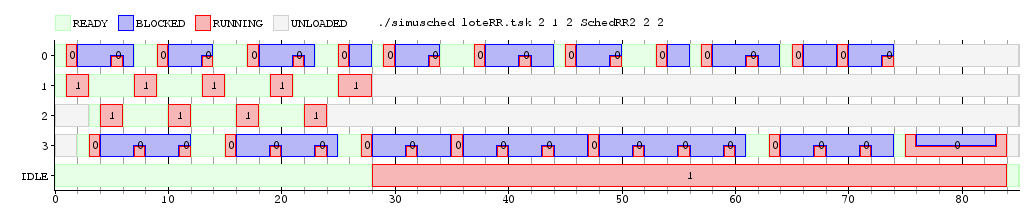
\includegraphics[width=\textwidth,height=3.0in,keepaspectratio
]{imagenes/ej8/2eje1.png} \newline
\begin {flushleft}
\textbf{Figura 12:} Diagrama de Gantt para la ejecuci\'on del lote de tareas bajo 2 n\'ucleos con quantums de 2 y 2 ciclos respectivamente. En un Scheduler Round Robin sin migración de procesos.
\end{flushleft}	
 
  
  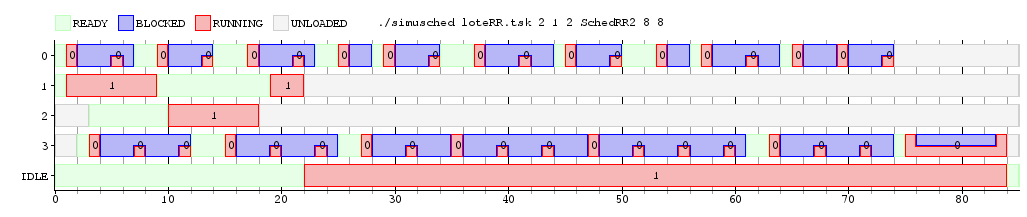
\includegraphics[width=\textwidth,height=3.0in,keepaspectratio
]{imagenes/ej8/2eje2.png} \newline
\begin {flushleft}
\textbf{Figura 13:} Diagrama de Gantt para la ejecuci\'on del lote de tareas bajo 2 n\'ucleos con quantums de 8 y 8 ciclos respectivamente. En un Scheduler Round Robin sin migración de procesos.
\end{flushleft}	

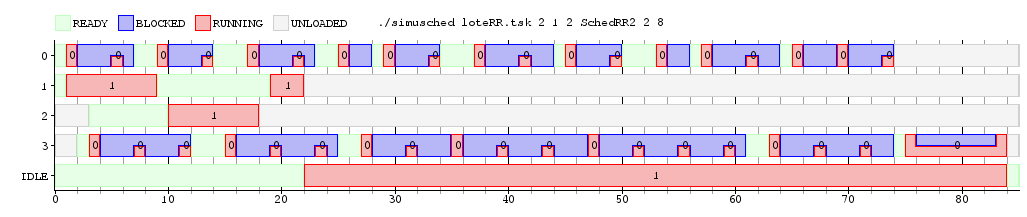
\includegraphics[width=\textwidth,height=3.0in,keepaspectratio
]{imagenes/ej8/2eje3.png} \newline
\begin {flushleft}
\textbf{Figura 14:} Diagrama de Gantt para la ejecuci\'on del lote de tareas bajo 2 n\'ucleos con quantums de 2 y 8 ciclos respectivamente. En un Scheduler Round Robin sin migración de procesos.
\end{flushleft}	

\bigskip
Y para las tareas: 
  
 \begin{codesnippet}
	\begin{verbatim}
 TaskCPU 7
@2:
TaskCPU 6
@1:
TaskCPU 10
@3:
TaskCPU 4
	\end{verbatim}
	\end{codesnippet}
	
Obtuvimos los siguientes resultados:\newline
	
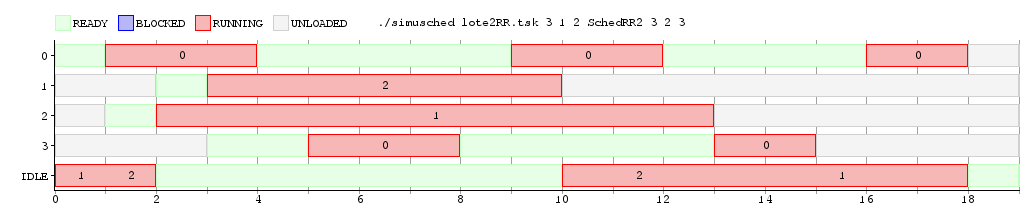
\includegraphics[width=\textwidth,height=3.0in,keepaspectratio
]{imagenes/ej8/2eje4.png} \newline
\begin {flushleft}
\textbf{Figura 15:} Diagrama de Gantt para la ejecuci\'on del lote de tareas bajo 3 n\'ucleos con quantums de 3, 2 y 3 ciclos respectivamente. En un Scheduler Round Robin sin migración de procesos.
\end{flushleft}	
	

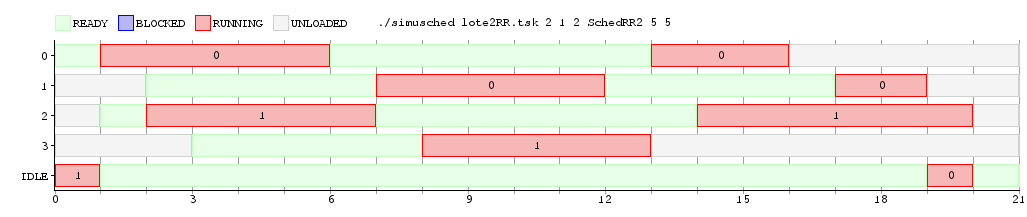
\includegraphics[width=\textwidth,height=3.0in,keepaspectratio
]{imagenes/ej8/2eje6.png} \newline
\begin {flushleft}
\textbf{Figura 17:}Diagrama de Gantt para la ejecuci\'on del lote de tareas bajo 2 n\'ucleos con quantums de 5 y 5 ciclos respectivamente. En un Scheduler Round Robin sin migración de procesos.
\end{flushleft}	
 
\newpage
 \subsection{Ejercicio 9:  Ejecuci\'on lote de tareas}
\textit{Dise\~nar un lote de tareas cuyo scheduling no sea factible para el algoritmo de prioridades fijas pero s\'i para el algoritmo de prioridades din\'amicas.}
\newpage
 \subsection{Ejercicio 10:  Ejecuci\'on lote de tareas}
\textit{Dise\~nar un lote de tareas, cuyo scheduling s\'i sea factible con el algoritmo de prioridades fijas, donde se observe un mejor uso del CPU por parte del algoritmo de prioridades din\'amicas.}




\end{document}

